\chapter{Chosen Index Structures and Hypothesis}
\label{chap:chosen-structures-hypothesis}
\centerline{\rule{149mm}{.02in}}
\vspace{2cm}

This section describes the structures which have been chosen to be implemented, in addition to the baselines described in Section \ref{sec:baselines}. The reasons for choosing these structures and the hypotheses that were made regarding their performance on the evaluation datasets will be discussed and defined.

\section{Abandoned Structure -- Splay Quadtree}

TODO: mention original plan of implementing the Splay quadtree???

\section{Pyramid Tree}
\label{sec:pyramid-tree-detail}

As described in Section \ref{sec:pyramid-tree}, the Pyramid tree reduces multi-dimensional points to one dimension, which can then be used in a one-dimensional index structure. The reason this structure has been chosen is because dimension reduction techniques have been found to perform well for high-dimensional data, compared to tree-based approaches \cite{md-structures-samet}. The original Pyramid-Tree paper showed good performance on uniformly distributed data and a real dataset (with the Extended Pyramid-Technique), when compared to Sequential Scan and the competitive X-tree \cite{pyramid-tree}. There are two fundamental differences between the focus of the paper's analysis and what this project is trying to achieve:
\begin{enumerate}
	\item the paper's analysis is for \textit{range} queries, whereas this project is primarily trying to accelerate point queries
	\item the real dataset, ``a large text database extracted from WWW-pages" \cite{pyramid-tree}, is a database containing discrete values, whereas the real datasets considered in this project are continuous, spatial, scientific datasets
\end{enumerate}
While the database dataset is of course mapped to a spatial domain, the data may have different properties or distributions than continuous, spatial-based data such as the astrophysics turbulence simulation. Therefore, it was decided that the Pyramid Tree shall be implemented to explore if the Pyramid Tree can provide equally good performance with point queries on these scientific datasets, in addition to the data being dynamic.

To elaborate on the reduction technique, the Pyramid tree partitions the data space into $2d$ Pyramids, where each is represented the $(d - 1)$ hyperplane corresponding to the Pyramid's base. Each pyramid is is segmented by splitting them along $(d-1)$ hyperplanes parallel to the base of the pyramid. The one-dimensional value of a point, called the \textit{pyramid value}, describes which Pyramid it is in and the height of that point in that Pyramid. The resultant spatial partition looks like Figure \ref{fig:pyramid-tree-buckets}, where each Pyramid segment has a corresponding bucket which stores the points.

\begin{figure}
		\begin{center}
			\begin{subfloat}[$2d$ Pyramids in 2D Data Space\label{fig:pyramid-tree-pyramids}]{%
				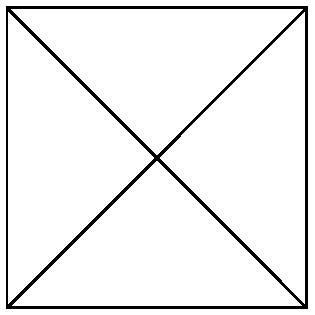
\includegraphics[scale=0.5]{figures/pyramid_tree_partition.pdf}
			}
			\end{subfloat}~
			\begin{subfloat}[Segmented $2d$ Pyramids, Each Associated with a Bucket\label{fig:pyramid-tree-buckets}] {%
				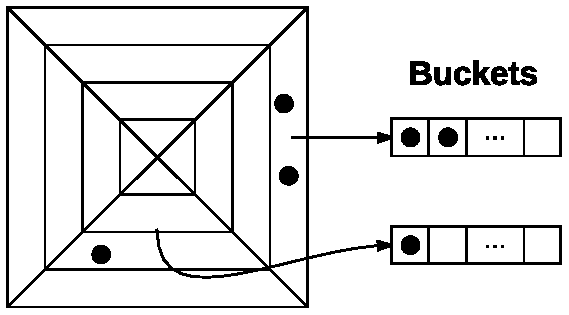
\includegraphics[scale=0.5]{figures/pyramid_tree_buckets.pdf}
			}
			\end{subfloat}
		\end{center}

		\label{fig:pyramid-tree-partition}
\end{figure}

More formally, the pyramid value $pv_v$ of a point $v$ is given by $pv_v = (i + h_v)$, where $i$ represents the pyramid $v$ is contained in and $h_v$ is height of $v$ in pyramid $i$. $i$ and $h_v$ are given in Equations \ref{eq:pyramid-value-index} and \ref{eq:pyramid-value-height} respectively, where $MOD$ refers to the modulo operator.

\begin{multline}\\
	i = \begin{cases}
		j_{max},         & \text{if }v_{j_{max}} < 0.5\\
		j_{max} + d,   & \text{if }v_{j_{max}} \geq 0.5\\
	\end{cases} \\
	j_{max} = \left( j \;|\; \forall k \; 0 \leq j,k \leq d, j \neq k: \;\; \lvert 0.5 - v_j \rvert \geq \lvert 0.5 - v_k \rvert \right) \\
	\label{eq:pyramid-value-index}
\end{multline}
\begin{equation}
	h_v = \lvert 0.5 - v_{i \; MOD \; d} \rvert
	\label{eq:pyramid-value-height}
\end{equation}

The following lemma shows that two distinct points can be mapped to the same Pyramid value. It follows that the Pyramid-technique as a hashing function may cause points to be stored in the same bucket. As such, bucket size will be a key performance factor for the structure and will be measured to provide a comparison to other hash-based structures discussed in this iteration.

\begin{proof}[\textbf{Lemma: } For $d \geq 2$, there exist two points $x$ and $y$, such that $x \neq y$, with the same pyramid value]\mbox{}\\*
Let $d$ be the number of dimensions and $x = (x_0, x_1, \dots, x_{d -1})$, $y = (y_0, y_1, \dots, y_{d - 1})$ be two $d$-dimensional points. Without loss of generality, assume $0 \leq x_i \leq 1$ and $0 \leq y_i \leq 1$ for all $i = 1, 2, \dots, d$. Suppose $x_0 = y_0 = 0$, $x_{d - 1} = 0.1$, $y_{d - 1} = 0.2$ and $x_i = y_i = 0.1$ for all $i = 1, \dots, {d - 2}$. This means $x \neq y$. The following holds:
\begin{enumerate}
	\item $\forall k \; 0 \leq k \leq d, k \neq 0: \;\; \lvert 0.5 - x_0 \rvert \geq \lvert 0.5 - x_k \rvert$,
	\item $\forall k \; 0 \leq k \leq d, k \neq 0: \;\; \lvert 0.5 - y_0 \rvert \geq \lvert 0.5 - y_k \rvert$.
\end{enumerate}
Since $x_0 \leq 0.5$ and $y \leq 0.5$, both $x$ and $y$ are mapped to pyramid 0 ($i = 0$). It follows that $h_x = h_y = \lvert 0.5 - v_{0 \; MOD \; 3} \rvert = \lvert 0.5 - v_{0} \rvert = \lvert 0.5 - 0 \rvert = 0.5$. $pv_x = pv_y = 0 + 0.5 = 0.5$ and $x \neq y$, meaning two distinct points can have the same Pyramid value.

\end{proof}

\section{Pseudo-Pyramid Tree}

The School of Computing have an implementation of an index structure which is similar to the Pyramid Tree, originally written by Zhao Geng\footnote{Z.Geng@leeds.ac.uk}. Like the Pyramid Tree, it reduces $d$-dimensional points to a single dimension, which is used to search for the original point in a one-dimensional search structure. Each 1D key has its own bucket that contains references to the original points which are mapped to it. Being another dimension reduction approach and have similarities to the Pyramid Tree, this will be implemented and evaluated alongside the other chosen structures. 

\begin{wrapfigure}[12]{r}{0.5\textwidth}
	\vspace{-40pt}
	\begin{center}
		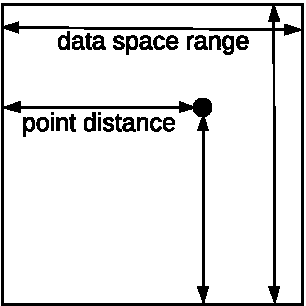
\includegraphics[scale=0.6]{figures/pseudo-pyramid_tree_point_boundary_distances.pdf}
	\end{center}
	\vspace{-20pt}
	\caption{Computing Distance of Point Along Pseudo-Pyramid Tree Boundary Along Each Dimension}
	\label{fig:point-boundary-distance}
\end{wrapfigure}

To determine if a point $p$ is stored in the structure, $p$ is first hashed into its one-dimensional representation. The corresponding bucket is then sequentially scanned until the point is found or the end of the bucket is reached. To reduce the number of floating point comparisons, especially for large $d$, the \textit{sums} of each point are stored when they are inserted. This way, a $O(d)$ point comparison needs to be made if the $O(1)$ point sum comparison passes. Simple optimisations were initially made to the original implementation. The original implementation passed many heap allocated structures by-value, resulting in excessive copies and more time being spent allocating memory and copying data. These copies were not necessary and were removed where possible by passing the data by-reference.

In this report, this variant of the Pyramid Tree shall be called the \textbf{Pseudo-Pyramid Tree}. This is because the hashing function used is \textit{inspired} by the Pyramid tree, but is not the same. Let $min_i$ and $max_i$ define the minimum and maximum bounds for dimension $i$ and $p$ be a point. To hash $p$, how far along the boundary $p$ is in each dimension is computed using Equation \ref{eq:point-boundary-distance} first. See Figure \ref{fig:point-boundary-distance} for an illustration of what these values mean.

\begin{equation}
	h_i(p) = \frac{p_i - min_i}{max_i - min_i}
	\label{eq:point-boundary-distance}
\end{equation}

Let $B$ be a parameter which controls how likely points will be in the same bucket and let $m$ be a point where $m_i = \ceil{B^{\frac{1}{d}}}$ for $0 \leq i \leq d$. The hashed value $h(p)$ of a point $p$ is then given by Equation \ref{eq:pseudo-pyramid-hash},  where \texttt{toInt} converts a real number to an integer by truncating the decimal part. Computing this is a $O(d^2)$ operation due to the inner loop to compute $\prod_{j=0}^{i}{\lbrack m_j \rbrack}$.

\begin{equation}
	h(p) = \sum_{i = 0}^{d} { \lbrack \texttt{toInt}( h_i(p) \times m_i ) \times \prod_{j=0}^{i}{\lbrack m_j \rbrack} \rbrack }
	\label{eq:pseudo-pyramid-hash}
\end{equation}

Higher $B$ means higher $m$. This increases the magnitude of $h_i(p)$ before it is truncated to an integer, meaning less points will have the same hashed value, meaning less points in the same bucket on average. Lower $B$ will therefore mean more points will be in the same bucket on average.

\section{$kd$-Tree}

The $kd$-Tree is a widely used structure for both low and high dimensional data. In the literature, there is a lot of discussion as to how and why this structure performs poorly in a high-dimensional setting \cite{highd-nn, search-highd-analysis}. This reveals that $kd$-trees are typically used for \textit{approximate} queries in higher-dimensional space, as they tend to degenerate to Sequential Scan for exact range and nearest neighbour queries \cite{similarity-searching}. 

Similar to the Pyramid Tree, the focus of the literature on $kd$-Trees is typically for range and nearest neighbour queries, and not point queries. Unlike the Pyramid Tree however, dynamic variants of $kd$-Trees have been explored much more (e.g. in \cite{bkd-tree, kdb-tree}), with the original paper proposing operations for incremental insertion and removal \cite{kd-tree}. The structure will be implemented because of it is dynamic and widely adopted in the field. Additionally, since the $kd$-Tree is a different class of index structure, not being a dimension reduction technique, a more comprehensive evaluation of the efficiency of all chosen structures can be produced.

$kd$-Trees will not be explained in more detail. The structure is a multi-dimensional binary tree, meaning it does not have the exponential memory requirements the Octree has. $kd$-Trees split the data space along a single dimension at each level of the tree (known as a level's \textit{cutting dimension}), instead of splitting by \textit{all} dimensions.

The variant of the tree implemented for this project contains one point per node and cycles through each dimension when choosing deciding which cutting dimension to use for each level of the tree. If $n$ is a $kd$-tree node, $i$ is the cutting dimension on that node's level and $p$ is the point stored in this node, then:
\begin{enumerate}
	\item $\forall q$ stored in the \textbf{left} subtree rooted at $n$: $p_i > q_i$ 
	\item $\forall q$ stored in the \textbf{right} subtree rooted at $n$: $p_i \leq q_i$.
\end{enumerate}
When inserting or querying a point $p$, the tree is traversed top-down in a similar fashion to a standard binary tree, by comparing $p_i$ to $n_i$, where $n$ is the point stored in the current node and $i$ is the cutting dimension of the current level.

% TODO: pseudo-code for this???
The \texttt{delete} operation used, described in \cite{kdtree-remove}, is more involved because it has to maintain the $kd$-tree invariant. To remove a point $p$, first the node containing $p$ is found using the aforementioned top-down traversal approach. Let $n$ be this node and $i$ be the current level's cutting dimension. If $n$ is a leaf, then the node can simply be deleted. Otherwise, let $n_L$ and $n_R$ be the left and right children of $n$ respectively. If $n_R$ exists, a node $m$ containing a point with the \textit{minimum} value for dimension $i$ is found in the sub-tree rooted at $n_R$. The points stored in nodes $n$ and $m$ are swapped and \texttt{delete($p$)} is called recursively on the sub-tree rooted at $n_R$. If $n_R$ does not exist, node $m$ is found in the sub-tree rooted at $n_L$ instead. In this case, after \texttt{delete($p$)} has been recursively called on the sub-tree rooted at $n_L$, the $i$th value of all points stored in this sub-tree are greater than or equal to the $i$th value of the new point in $n$. Therefore, $n_L$ then becomes the \textit{right} child of $n$ to maintain the $kd$-tree invariant. 

Figure \ref{fig:kd-tree} illustrates the \texttt{insert} and \texttt{delete} operations.

\begin{figure}
	\begin{center}
		\makebox[\textwidth][c]{
		\begin{subfloat}[Inserting Point $(3, 1)$\label{fig:kdtree-insert}]{%
			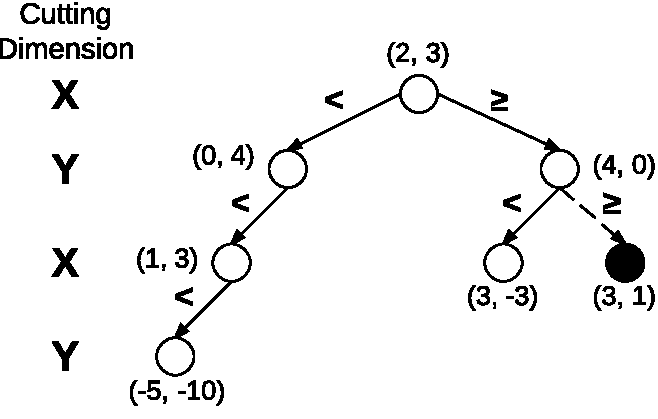
\includegraphics[scale=0.5]{figures/kdtree_insert.pdf}
		}
		\end{subfloat}~
		\begin{subfloat}[Deleting Point $(0, 4)$\label{fig:kdtree-delete}]{%
			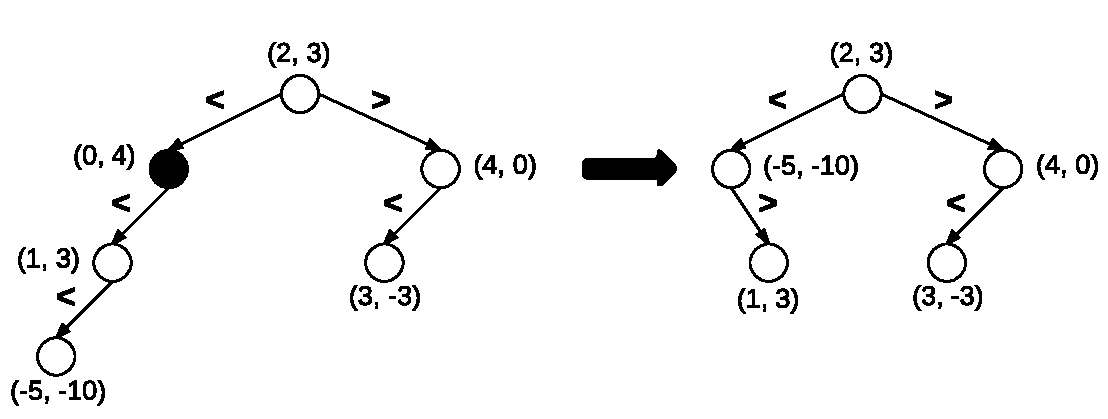
\includegraphics[scale=0.5]{figures/kdtree_delete.pdf}
		}
		\end{subfloat}	  
		}%
	\end{center}

	\caption{$kd$-Tree Operations for 2D Dataset (Cutting Dimension Alternates Between X and Y)}
	\label{fig:kd-tree}
\end{figure}

\section{Main Hypothesis}
\label{sec:main-hypothesis}

Since there has been no published evaluations of the Pseudo-Pyramid Tree, no hypotheses will be made regarding the performance of the structure. It is suspected that the Pseudo-Pyramid Tree will perform well on high-dimensional data, because it is a hash-based method, but little is currently known about how well the structure's hashing function performs, so there is a little basis for such suspicion. Before starting implementation, the following hypothesis regarding the Pyrmid Tree and $kd-Tree$ was devised:

\paragraph{\textbf{HYPOTHESIS:}} Pyramid Tree will be faster than the baselines and $kd$-Trees on all evaluation datasets containing high-dimensional data ($\geq 10$ dimensions).

\paragraph{}

This hypothesis was based on the reported performance of the Pyramid Tree and $kd$-Tree in a high-dimensional setting in the literature, as discussed in the previous sections. After the implementation phase, the hypothesis will be revisited to determine if it still holds, and \textit{why} it does or does not hold will be explored.